\chapter{Experiments and Results}
\label{cha:experiments_and_results}

In this chapter obtaining results from the MA will be considered. First there will be a section that looks into the results one gets when the MA is applied to the BHW1 benchmark \citep{BHWdocumentationSINTEF}. Because the smaller BHW instances are solved to optimality, this will give an idea of the MAs performance relative to known optimal solutions. Then there will be a section about obtaining results when map data from Trondheim is used as input to the MA.

\section{The BHW Benchmark}
\label{sec:the_bhw_benchmark}

Here the MAs performance on the BHW1 test case is going to be presented. Because the BHW1 benchmark has been solved optimally, and the solution is available, it can be used to verify the output of the MA. When comparing the fitness of the result from the MA with the fitness of the know solution one should be able to gauge the quality of the MAs output. And when observing the optimal route with the one made by the MA it should become apparent whether the MA is on the right track or not.

The section will start out by outlining the experimental plan for the tests. After the experimental plan has been given, the experimental setup will be described. And finally the results of the tests will be presented.

\subsection{Experimental Plan}

To be able to compare the routes generated by the MA and the known solution for the BHW1 case and their fitnesses, clearly a result form running the MA on the BHW1 benchmark has to be obtained. The generated route and the known solutions' route should be displayed side by side, and the fitness the MA finds should be compared to the fitness of the solution.

\subsection{Experimental Setup}

To be able to compare the fitness and the rsulting routes produced by the MA with the known solution, the MA should be set to process the BHW1 case. The result should be compared to the one found on \citet{BHW1Solution}.

To get an idea of what fitnesses the MA genereally finds when processing the BHW1 case, it will be run 30 times for 50000 generations with the parameters shown in table \ref{tab:BHW1_params_table}. The fitness evaluation will be performed by evaluating the sum of the lengths of the splitted trips generated from each genome, due to that being how the fitness of the optimal solution is calculated. After having preformed the series of runs, the result from the best run is going to be picked and compared to the known solution.

{
\rowcolors{2}{gray!15}{white}
\begin{table}[tbph]
\centering
\begin{tabular}{ll}
\toprule
\textbf{MA Parameter} & \textbf{Setting to be Used}     \\ \midrule
Parent selection      & Fitness proportionate selection \\
Adult selection       & Overproduction                  \\
Mutation type         & Memetic improvement             \\
Population size       & 90 individuals                  \\ \bottomrule
\end{tabular}
\caption{The parameters used for testing the MA on the BHW1 benchmark.}
\label{tab:BHW1_params_table}
\end{table}
}

\subsection{Results}

After running the MA on the BHW1 benchmark with the parameters described above, the average of the best, average, and standard deviation of fitness of the populations each generation were plotted. The charts can be seen in appendix \ref{cha:bhw1_benchmark_results}. From the cart in figure \ref{fig:bhw1ab}, it can be seen that the best solutions the MA finds have a fitness of about 370.

The best result obtained was the run labeled as 2015-06-24T01-34-22Z, which can be found in the supplementary digital materials. It had a fitness of 360, which compared to the optimal fitness that is 337 is completely fine. The trips found by the MA and and the optimal trips from \citet{BHW1Solution} can be seen in table \ref{tab:BHW1_solutions_compared}. As can be seen in the table, the trips found by the MA show resemblance to those of the optimal solution. For an instance the first part of the fourth trip found by the MA is very similar to the first part of the third trip of the optimal solution.

{
\rowcolors{2}{gray!15}{white}
\begin{table}[tbph]
\centering
\resizebox{\textwidth}{!}{
\begin{tabular}{lll}
\toprule
                & \textbf{Result from MA}                         & \textbf{Known Optimal Solution} \\ \midrule
\textbf{Trip 1} & 1-A5-N12-E8-N12-A9-6-E4-6-N12 1                 & 1-A1-N2-E3-9-A11-11-E5-5 1     \\
\textbf{Trip 2} & 1-A1-N2-E3-9-A11-N11-E9-8-A10-N10-E10-9-E3-N2 1 & 1-A2-4-E2-2-E1-N3 5-E6-12 1    \\
\textbf{Trip 3} & 1-A2-N4-E2-N2-E3-N2-E1-N2 1                     & 1-A4-10-E11-N11-E9-8 7-E8-12 1 \\
\textbf{Trip 4} & 1-A4-N10-E11-N11-E5-5-E4-6-N12 1                & 1 12-A9-6-E4-5-A7-3-A6-N4 1    \\
\textbf{Trip 5} & 1-A3-N7-E7-N7-A8-6-N12 1                        & 1-A3-7-E7-8-A10-N10-E10-9 1    \\
\textbf{Trip 6} & 1-A5-N12-E6-5-A7-N3-A6-N4 1                     & 1-A5-N12 N7-A8-6 1             \\ \midrule
\textbf{Fitness}    &    \textbf{360}    &    \textbf{337}    \\ \bottomrule

\end{tabular}
} %close resizebox
\caption{The best result obtained from the MA and the known optimal solution for the BHW1 benchmark.}
\label{tab:BHW1_solutions_compared}
\end{table}
}

\section{Map Data from Trondheim}
\label{sec:map_data_from_trondheim}

Now that it has been established that the MA works (as shown in chapter \ref{cha:evolutionary_algorithm_configuration}), and produces results of a reasonable quality when applied to benchmark problems (detailed in chapter \ref{sec:the_bhw_benchmark}), RQ3 should be addressed. RQ3 was stated in table \ref{tab:research_questions} as: \enquote{Determine whether the memetic algorithm independently can find a route in Trondheim optimized for length weighted by speed with a random starting point}.

To properly test whether the MA can routes in Trondheim, it should be applied to map data form Trondheim. This section will start out by exploring what data should be gathered to properly deal with RQ3. Then the experiments used to obtain the data will be detailed. Finally after that the results obtained from the experiments will be outlined.

\subsection{Experimental Plan}

To get results on the performance of the MA when trying to create snow plowing routes for Trondheim, clearly it should be fed a graph that is generated from road map data of Trondheim. To check whether the MA is consistently capable of finding solutions it should be run a number of times, and the quality of the results in terms of their fitness should be plotted.

Once the MA has generated a set of results, these results should be compared to the routes currently being driven. To do this the fitnesses of the generated routes should be compared to the fitness the implementation calculates for the routes as they are driven. This way they will both be evaluated in terms of a common refference frame, the model based on the map data from Trondheim.

Then the routes generated by the MA should be drawn up as a map. It could be argued that they should be drawn \emph{on} a map, but due to copyright issues and the nature of the process of generating map tiles it is not feasible to do at this point in time. When the routes have been drawn up, they can visually be inspected for flaws and abnormalities. Additionally having the routes presented graphically is usefull if they are to be applied in a real life setting by a snow plow driver.

The drawn routes generated by the MA could also then be evaluated by the municipalitys drivers. This could bring to light aspects of the generated routes that might otherwise be overlooked, and their assessment can also be used as a way to evaluate the quality of the generated routes.

\subsection{Experimental Setup}

To produce snow plowing routes for Trondheim the MA needs to be supplied a graph of the area with the streets that need to be plowed, as discussed in chapter \ref{architecture_and_implementation}. An important feature of the chosen NEARP format should be considered here, namely that it requires a starting point be specified (in the \enquote{depot node}-field). Due to that the route being generated for the actual snow plowing case is a giant circle, the starting point is somewhat arbitrary. It will add to the length of the route, because the MA connects it to the cycle. But because the connection is the shortest path to the cycle, and it will be the same for all routes, it should not have to great of an influence. It can be argued that the choice of starting point will affect where the cycle begins, but because that does not change the nature of the cycle otherwise it should not matter and the starting point can be chosen arbitrarily. Therefore the starting point for each route is chosen to be the first required element appearing in the input.

To generate the routes then, the MA will be configured with the parameters shown in table \ref{tab:trondheim_params_table}. It will be applied to two sets of roads that need to be plowed in existing routes; route 310174\_KV\_B\_Midtbyen, and route 310179\_KV\_H\_Midtbyen. To get an idea about its performance in general it will be run 30 times with this configuration. Ten of the runs are going to be 100000 generations long, to illustrate how the results converge over time. The remaining 20 runs will be going for 50000 generations, and the average performance will be graphed based on the first 50000 generations of all 30 runs combined.

{
\rowcolors{2}{gray!15}{white}
\begin{table}[tbph]
\centering
\begin{tabular}{ll}
\toprule
\textbf{MA Parameter} & \textbf{Setting to be Used}     \\ \midrule
Parent selection      & Fitness proportionate selection \\
Adult selection       & Overproduction                  \\
Mutation type         & Memetic improvement             \\
Population size       & 200 individuals                 \\ \bottomrule
\end{tabular}
\caption{The parameters used when applying the MA to map data from Trondheim.}
\label{tab:trondheim_params_table}
\end{table}
}

To get the fitness of the routes as they are currently being driven for comparison with the generated routes, the municipalitys drivers will be asked to supply a list of what order they clear the roads on their route in. The lists are then going to be processed by looking up each of the enumerated road elements in the model of the road network data from Trondheim stored in QGIS. There the IDs of the elements will be obtained, and written down in a file. This file will then be formated so that it represents a route in the internal format used by the MA, by prepending each element ID with an \enquote{E}, \enquote{A}, or \enquote{N} to denote whether it is an edge, arc, or node respectively. Then each item will be wrapped in double quotes ("), and separated with a comma (,) so that it can be properly parsed as an array by the MA.

A similar process is going to be used when the resulting routes are drawn as maps. Instead of adding characters to denote whether an element is a node, edge, or arch, all extra characters except the numerical IDs of the elements and delimiters will be stripped. The resulting list is then going to be fed to QGIS in the form of a csv-file, where a graphical representation of it will be made. Finally a meeting with the municipality and the snow plow drivers will be set up so that feedback on the results from domain experts can be presented.

\subsection{Results}
Show some nice graphs of how the fitness converges over time.
Show a created map, and refer to tiles with finer details in the appendix.
Show how the fitness of the pre-existing routes relates to the fitness of the calculated ones.
Discuss how the system does som smart things that humans would perhaps not (cover the city in a set of veird overlapping sections), how some interesting behavior like driving into a road, servicing it, and then driving back out the same end as it was started in and continue that route arises. Also highlight some missed one way roads and gaps in the map.



The charts showing how the MA behaves when run for 100000 generations can be seen in the figures in appendix \ref{cha:gotpotmwatmdft}. From figures \ref{fig:KV_B_100k_aa} and \ref{fig:KV_H_100k_aa} it comes forth that the algortihm generally tends to stabilize after 10000 generations, and figures \ref{fig:KV_B_100k_ab} and \ref{fig:KV_H_100k_ab} show that there is little improvement in the best found solution after that point. In the charts showing the combined results of the MA running for 50000 generations and 100000 generations when the first 50000 generations are plotted, one can find the fitness at which the MA tends to converge to at 50000 generations. For route 310174\_KV\_B\_Midtbyen the best fitness found on average has a value of 564882 which can be seen in figure \ref{fig:KV_B_50k_ab}, and for route 310179\_KV\_H\_Midtbyen the average best fitness after 50000 generations is 411770, as seen in \ref{fig:KV_H_50k_ab}.

The overall best fintesses obtained for each route, and the fintesses of how they are being driven at the present can be seen in table \ref{tab:trondheim_data_fitness_comparisons}. For route 310174\_KV\_B\_Midtbyen the fitness of the route generated by the MA is 35\% smaller than the fitness of how the route is currently being driven, which is signifficantly better. When looking at route 310179\_KV\_H\_Midtbyen, one finds that the fintess found by the MA is 50\% smaller than the driven one. From this it can be concluded that as long as one assumes that the model is valid, the MA, although not capable of finding optimal solutions, is able to find solutions better than the ones made by humans.


{
\rowcolors{2}{gray!15}{white}
\begin{table}[tbph]
\centering
\resizebox{\textwidth}{!}{
\begin{tabular}{cp{0.36\textwidth}p{0.36\textwidth}}
\toprule
\textbf{Route}          & \textbf{Fitness of route generated by the MA} & \textbf{Fintess of the route as it is driven currently} \\ \midrule
310174\_KV\_B\_Midtbyen & 444632 & 685933 \\
310179\_KV\_H\_Midtbyen & 306060 & 617670 \\ \bottomrule
\end{tabular}
} %close resizebox
\caption{The best result obtained from the MA and the known optimal solution for the BHW1 benchmark.}
\label{tab:trondheim_data_fitness_comparisons}
\end{table}
}

But other than evaluating the routes by their fitness values, they should also be visually inspected to check for anomalities that might not have been caught so far in the process. A graphical representation is also usefull if the generated routes are to be applied by drivers in practice. The maps drawn for the generated routes have therefore been made, and are presented in figures \ref{fig:KV_B_drawn} and \ref{fig:KV_H_drawn}, for routes 310174\_KV\_B\_Midtbyen and 310179\_KV\_H\_Midtbyen respectively. The route mapped for 310174\_KV\_B\_Midtbyen had a fitness of 515610, and the one used to generate the map for the 310179\_KV\_H\_Midtbyen route had a fintess of 472610.

In the figures, the numbers represent the order in which a road piece is visited. If one observes the maps carefully, it can be seen that there are some numbers that are missing. There are several reasons for this. First and foremost, some of the road pieces are very small, and labeling them would make the label collide with the labels of adjacent road pieces if one does not use a text size so small that it would be practically unreadable. Another factor that makes displaying the complete enumeration difficult is that some roads are traversed several times. Coupled with an already limited space to display the labels, this makes even more labels disappear. To show all the labels, one would have to print the map on A0 paper with a font-size of 4 points.

The practical solution was to print with the size and resolution used in the figures. The are humanly readable, and it is relatively easy to infer the missing numbers upon inspection. For completeness the maps have been generated with a finer resolution (40 times 40 meters) in the style of a map book that spans several pages. For route 310174\_KV\_B\_Midtbyen the detailed map can be found in appendix \ref{sec:detailed_generated_map_for_route_310174_kv_b}, and for the 310179\_KV\_H\_Midtbyen route in appendix \ref{sec:detailed_generated_map_for_route_310179_kv_h}. They are also available digitally as interactive maps formated for QGIS in the supplementary materials.

\begin{landscape}
\begin{figure}[thbp]
	\centerline{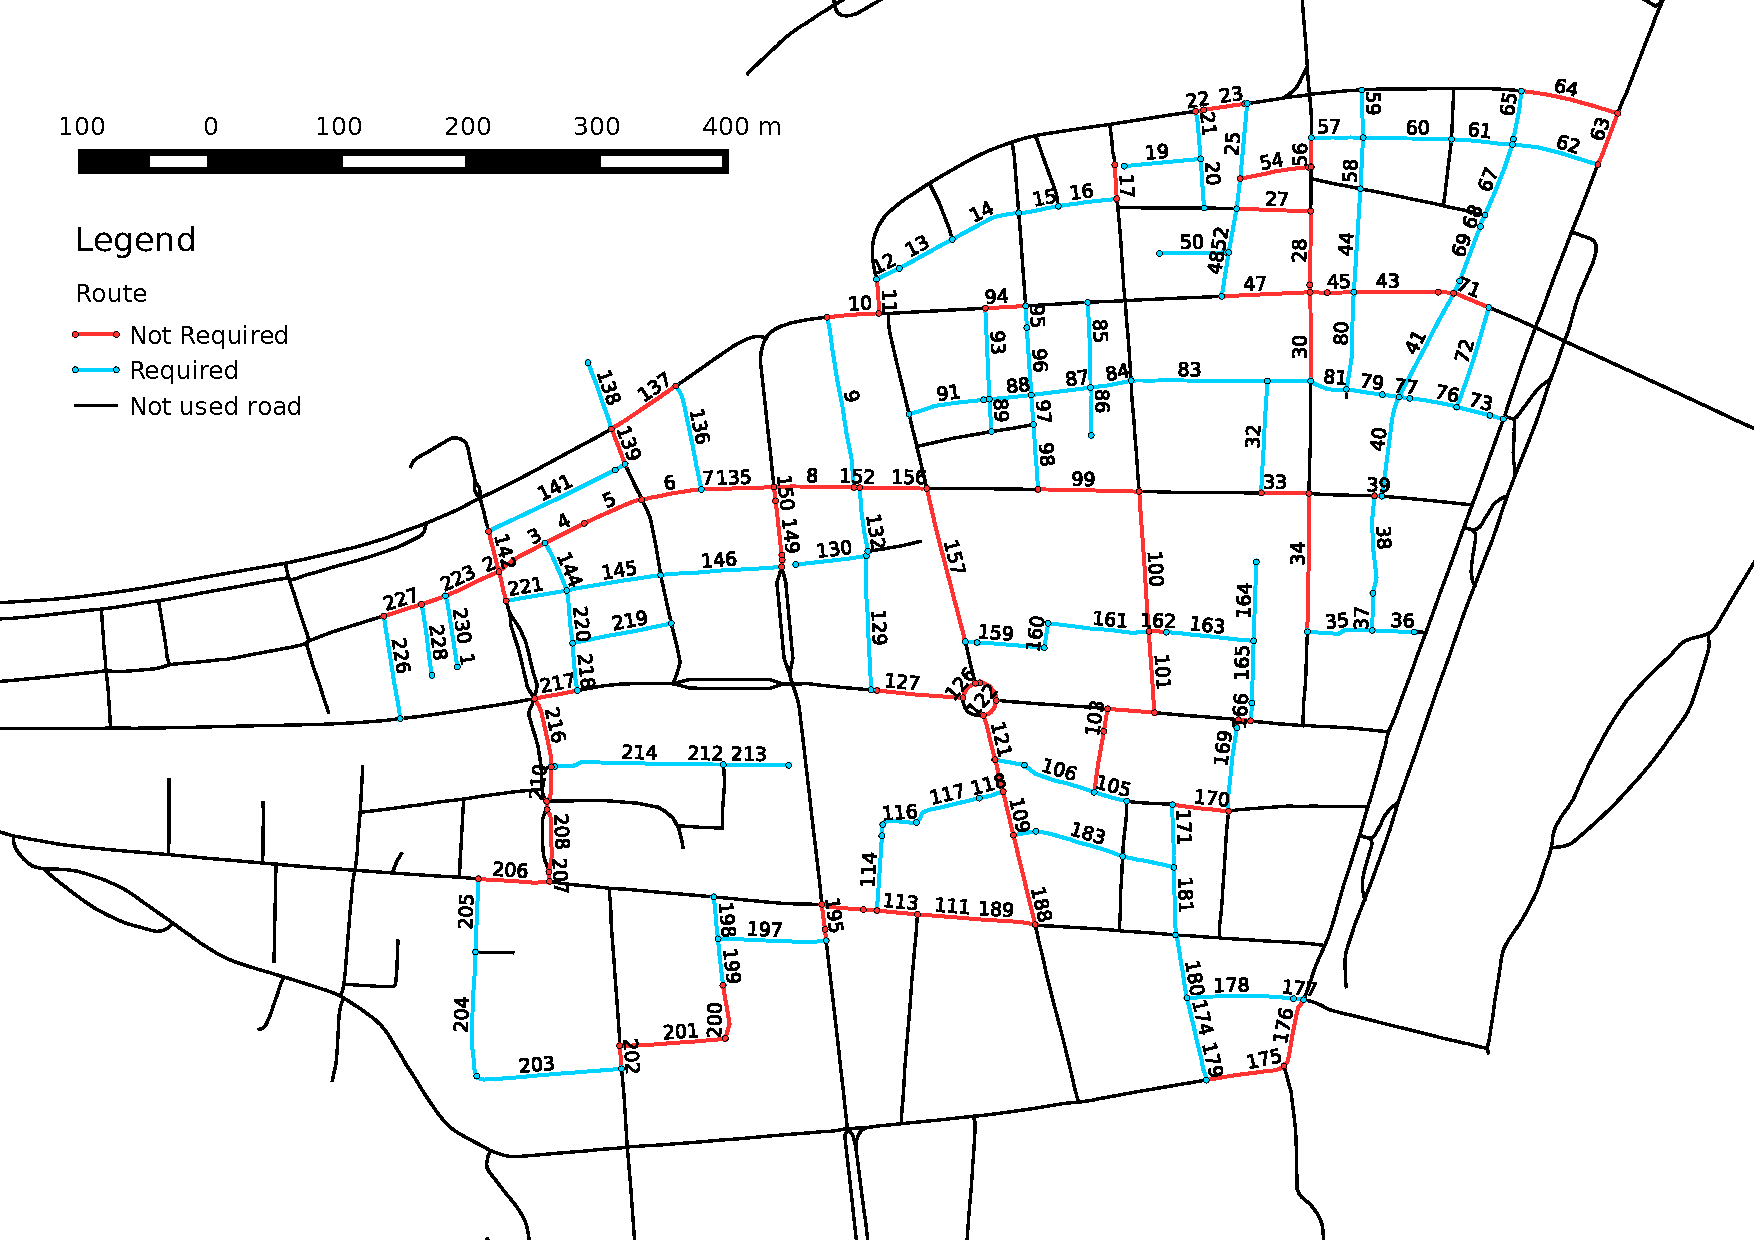
\includegraphics[height=0.945\textwidth]{figures/Routes/Drawn/Rute_KV_B_Generert_Proper_Run.pdf}}
	\caption{Route 310174\_KV\_B\_Midtbyen Generated by the MA}
	\label{fig:KV_B_drawn}
\end{figure}
\end{landscape}

\begin{landscape}
\begin{figure}[thbp]
	\centerline{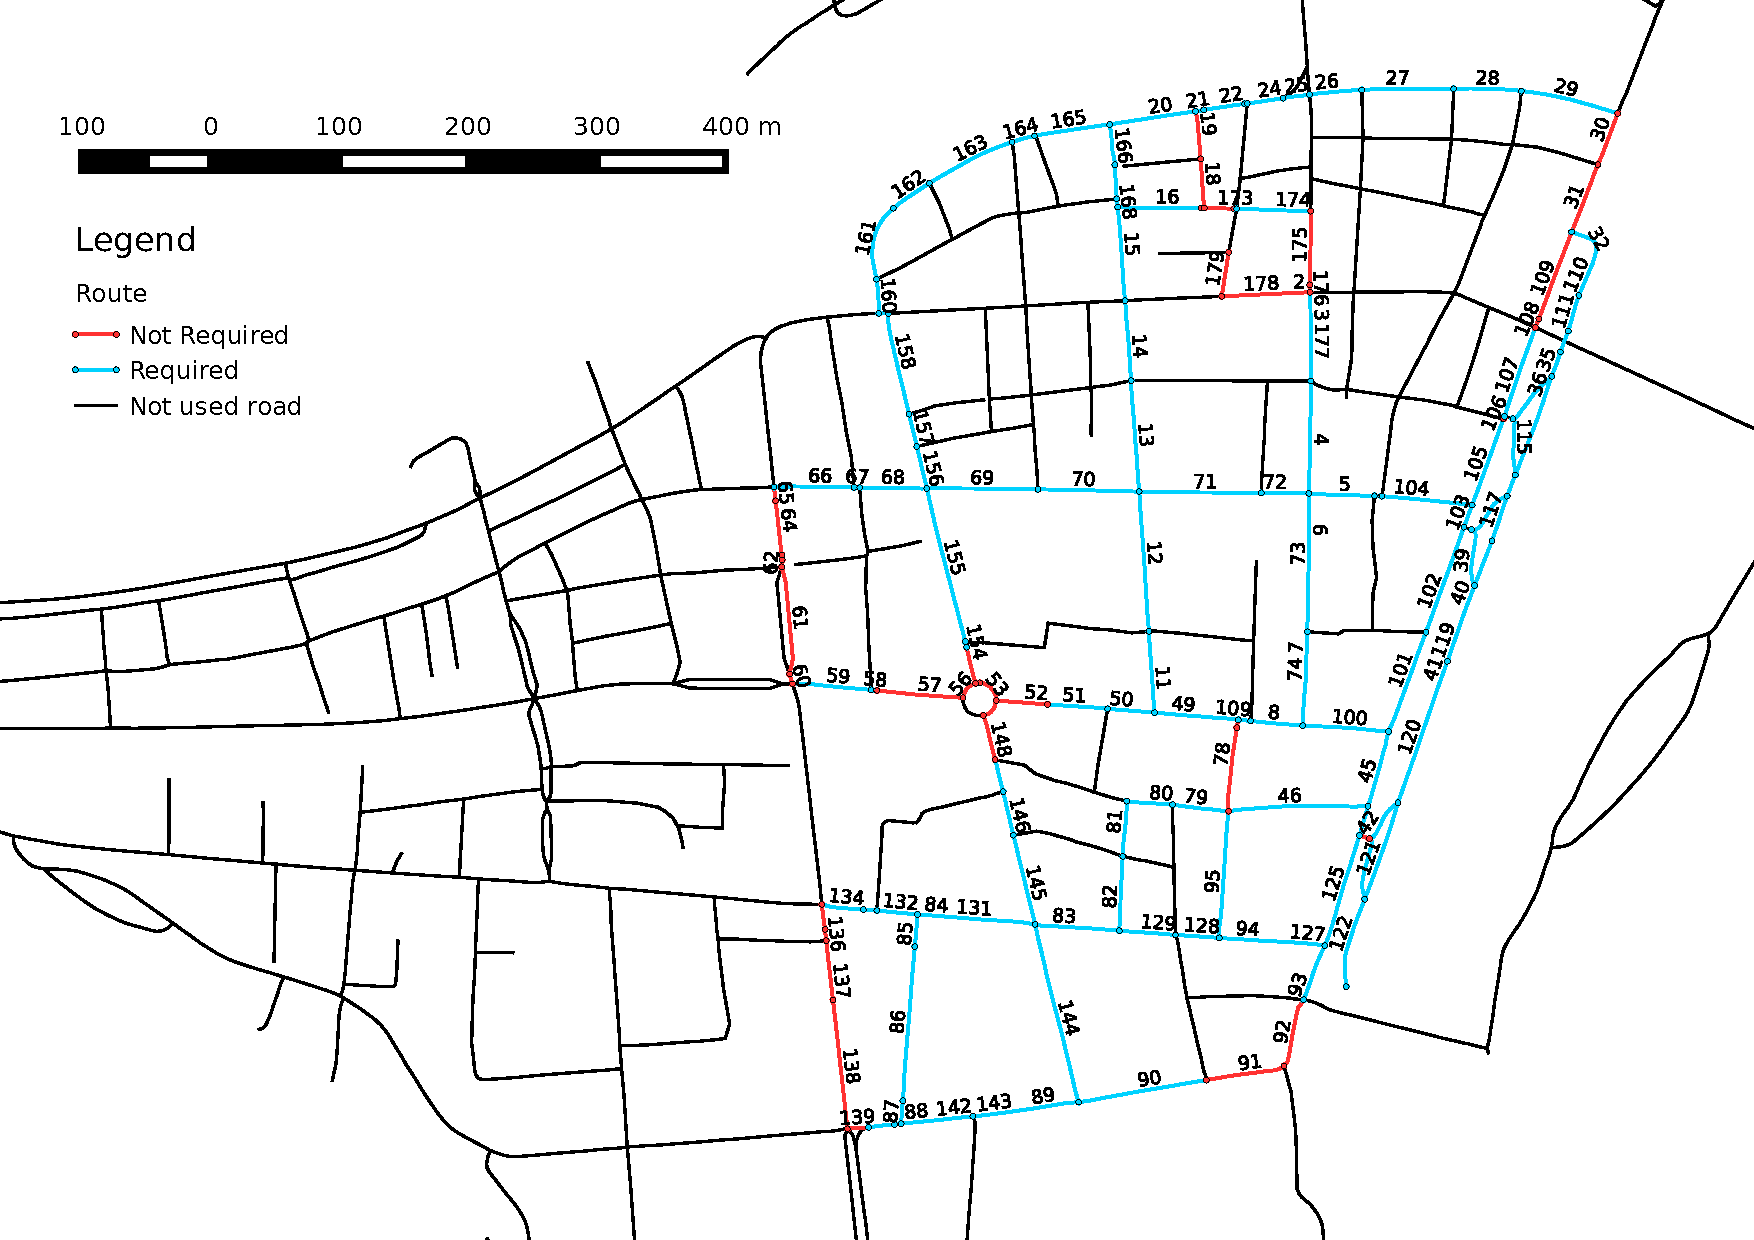
\includegraphics[height=0.945\textwidth]{figures/Routes/Drawn/Rute_KV_H_Generert_Proper_Run.pdf}}
	\caption{Route 310179\_KV\_H\_Midtbyen Generated by the MA}
	\label{fig:KV_H_drawn}
\end{figure}
\end{landscape}

Another interesting thing to observe is that some pieces of road appear to be missing, but still used, such as the pieces at about (9207510\degree N,1157400\degree E) and (9207120\degree N,1157190\degree E) in the route for 310174\_KV\_B\_Midtbyen (shown in the second and twelfth tiles of the extended map in \ref{sec:detailed_generated_map_for_route_310174_kv_b} respectively). Initially, one might believe that the pieces of road are missing due to errors in the underlying data or have gone missing during the processing. However, the fact that the apparently missing pieces are the only possible entities that can hold the corresponding values that are not shown in the routes at those points indicates that the fault does not lie in the underlying data. Instead, it must be an error in how the data is displayed. Fortunately it would seem that it has no effect on the readability of the routes or the correctness of the input and output of the MA.

To get a more thorough assessment of the drawn routes and some feedback on how well the visualization would work in practice, a meeting with the municipality and their snow plow drivers was set up \citep{meetingToAssesTheGeneratedRoutes}. There the maps as they were drawn in figures \ref{fig:KV_B_drawn} and \ref{fig:KV_H_drawn} was presented, alongside the interactive versions in QGIS to facilitate more detailed inspection of the routes.

Overall they found the representation satisfactory. It was pointed out that the drawn maps should have less details to be more convenient to use in practice. While having each road be represented as relatively small pieces makes sens for maintaining details and integrity of the map data over time, it serves no use when the drivers are reading the maps. Their conclusion was that it would be better if each road was represented and numerated as one piece between intersections, although the representation in figures \ref{fig:KV_B_drawn} and \ref{fig:KV_H_drawn} is completely legible and fine to use for evaluation.

Upon closer inspections of the maps, some new anomalities were also discovered. For an instance the road pieces labeled as number 211 to 215 in route 310174\_KV\_B\_Midtbyen are driving in and out of a one way driven alley, which should clearly not be done. It was discovered that the road pieces were not labeled as one way driven in the map data passed to the MA. Similarly in route 310179\_KV\_H\_Midtbyen the road pieces traversed as items number 53 to 56 and 148 to 152 in the big roundabout in the center of the town should be inaccessible to the vehicle used for servicing that route. The entire square in which the roundabout lies, although still maintained as part of the road network, and therefore in the underlying map data, has been blocked for traffic.

However the drivers assessed that these were minor flaws that were easy to work around. In their usual work, they said, it often happens that a particular street or alley is blocked by for an instance delivery vehicles. Then they have to drive out the way they came and around. Or if they are to service that end of the road they might have to go and plow other places and remember to come back later.

Another thing that was brought up at that point was that the route generated by the MA does not take into account that certain roads might need to be traversed several times before they are properly cleared of snow. But this was also dismissed as a minor flaw in their eyes, because while it to some extent depends on the width or the road, it also varies with the quality of the snow, amount of snow, traffic, etc.

From all this it can be seen that the MA manages to create routes based on data from Trondheim which can be presented in a meaningfull way to those that would use them. And although the routes may have flaws, they are still deemed to be usable in practice, and an interesting take on how the work can be performed by the drivers.

\cleardoublepage
